%\documentclass[11pt, onecolumn, conference]{IEEEtran}
\documentclass[conference]{IEEEtran}
\IEEEoverridecommandlockouts
% The preceding line is only needed to identify funding in the first footnote. If that is unneeded, please comment it out.
\usepackage{cite}
\usepackage{amsmath,amssymb,amsfonts}
\usepackage{algorithmic}
\usepackage{graphicx}
\usepackage{textcomp}
\usepackage{xcolor}
\usepackage{array}
\def\BibTeX{{\rm B\kern-.05em{\sc i\kern-.025em b}\kern-.08em
    T\kern-.1667em\lower.7ex\hbox{E}\kern-.125emX}}
\begin{document}

\title{Distributed Mutual Exlcusion Algorithms: A Comparison of Central Server,
Ring Token and Multicast\\
{\footnotesize COMPSYS 725: Distributed Cyber-Physical Systems}
}

\author{\IEEEauthorblockN{Matt Eden}
\IEEEauthorblockA{\textit{Department of Electrical, Computer and Software
Engineering} \\
\textit{University of Auckland}\\
Auckland, New Zealand \\
mede607@aucklanduni.ac.nz}
}

\maketitle

%\begin{abstract}
%\end{abstract}

%\begin{IEEEkeywords}
%central server, ring token, multicast, mutual exclusion, distributed systems
%\end{IEEEkeywords}

\section{Mutual Exclusion Algorithms}
\subsection{Overview}
Mutual exclusion is generally concerned with preventing interference and
ensuring consistency with resource access. For operating systems, this can be
managed with relative ease. However, distributed systems do not have the
shared variables or facilities that would be supplied by a single local kernel,
so a different approach is required. This is where distributed mutual exclusion
algorithms come into play, and a few of these are discussed in the following
subsections. \\
There are a few key assumptions made in this report that should be
acknowledged. The system being considered is comprised of \textit{N} processes
\textit{p\textsubscript{i}} with $i=1,2,3... N$. These process do not share
variables, but access common resources. These resources are contained within
a single critical section, and the system as a whole is asynchronous. The
failure of processes is not considered, with message delivery being reliable so
that any message sent is guaranteed to be delivered eventually and delivered
exactly once. 
\subsection{Comparing Algorithms}
The requirements for mutual exclusion considered in this report are:
\begin{itemize}
  \item Safety [ME1]
  \item Liveness [ME2]
  \item Fairness [ME3]
\end{itemize}
\textit{Safety} is concerned with the idea that at any instant in
time only one process may occupy the critical section. \textit{Liveness} is
concerned with the idea that any and all requests to enter the critical section
will eventually succeed. \textit{Fairness} is concerned with
how processes enter the critical section according to the order of requests. In
this report I consider the `happened-before' approach, wherein if one request
to enter the critical section `happened-before' another, then the entry is
granted in that order.
In addition to satisfying the above, performance of any one algorithm is evaluated against a set of fixed criteria,
defined as follows.
\begin{itemize}
  \item Consumed Bandwidth
  \item Client Delay
  \item Synchronisation Delay
\end{itemize}
The \textit{Consumed Bandwidth} is proportional to the number of the messages
sent in \texttt{entry()} and \texttt{exit()} (as defined previously).
\textit{Client Delay} is the time taken by a process at each \texttt{entry()}
and \texttt{exit()}. \textit{Synchronisation Delay} is simply the time
difference between one process' \texttt{exit()} and another's \texttt{entry()}.
\subsection{Central Server}
The simplest algorithm described in this report consists of a central server
managing requests for mutual exclusion from several processes. The overarching
idea is that a token is held by this central server, loaned out to a process
that has requested to enter the critical section and then retrieved once that
process leaves the critical section. The central server maintains a record of
requests it has received, and allocates tokens accordingly. The resolution of
a request involves removing said request from the queue and allocating the
token to that process. This workflow is illustrated in
Figure~\ref{fig:central-server}, where \textit{p\textsubscript{2}} is making
a request to the server for the token, \textit{p\textsubscript{3}} is releasing the token
it held back to the server and \textit{p\textsubscript{4}} is being allocated
the token by the server as. Infer from the diagram that
\textit{p\textsubscript{3}} had previously made a request and obtained the
token from the central server, hence why it is now releasing the token back to the
server. Similarly, \textit{p\textsubscript{4}} must have previously made
a request to the central server as it is higher in the queue than
\textit{p\textsubscript{2}}. \\
This algorithm satisfies ME1 because, due to the inherent nature of the design,
only one process can enter the critical section at a time. This is a direct
result of the central server only allocating a single token, as when one
process holds the token it cannot be allocated to any other process. ME2 is
also satisfied by this algorithm, as a simple first-in first-out (FIFO) queue
is used to order the requests by processes. Such an approach ensures the
eventual allocation of a token to any process that requests it. \\
However, ME3 is not satisfied by the central server algorithm. The reason being
that the ordering of requests is based purely on when the central server
receives the request, not when the request itself is sent. As such, there is no
guarantee that the `happened-before' relationship is satisfied.
\subsection{Ring Token}
This approach does away with the dependence on a third-party element as seen in
the central server algorithm, instead choosing to arrange processes in
a logical ring. In doing so, the requirement is introduced that each process
possesses a communication channel with the next. The token-based approach to
allowing access to the critical section continues, with the token passed along
the ring as illustrated in Figure~\ref{fig:ring-token}. Upon receiving a token,
a process may take one of two actions. Either it (a) enters the critical
section or (b) passes the token to the next process. If a process has requested
to enter the critical section then it peforms the former, otherwise it takes
the latter.\\
This algorithm satisfies ME1 due to the round robin approach taken meaning that
two processes cannot execute in the critical section at the same time. There is
only a single token that is passed round, therefore only one process executing
in a critical section. ME2 is satisfied for similar reasons, as the token is
being continously passed around the ring each process will eventually gain
access to the critical section (even in cases where it did not request it). ME3
is however not satisfied, as the clockwise rotation of the token goes against
the `happened-before' approach. A process \textit{p\textsubscript{N}} may make
a request, but as the token is being passed through the ring another process
\textit{p\textsubscript{N-2}} may similarly make a request. As the token
reaches the second process first, even though the request was made afterwards,
ME3 is not satisfied.
\subsection{Multicast}
The last algorithm discussed in this report, the multicast approach aims to
address the issues of the previous two algorithms. Namely, it attempts to
satisfy all three properties ME1, ME2 and ME3. Fundamentally, multicast works
based on waiting for a response by all other processes to a request made by
one process that wishes to enter the critical section. This is illustrated in
Figure~\ref{fig:multicast}, with the connections between nodes on the graph
representing the reponses and requests made. To assist in this approach,
Lamport clocks and timestamps are employed. It is assumed both that all
processes have communication channels with one another and self-identify
through the use of numerical IDs and timestamps. Each process has
a \textit{state}; either \textit{WANTED}, \textit{RELEASED} or \textit{HELD}.
These correspond to wanting the token, no longer needing the token and holding 
the token.
When multiple processes issue a request close in time to each other, the one
with the lowest Lamport timestamp is the first to collect replies and therefore
first to execute in the critical section. \\
This algorithm satisfies ME1 as a process cannot execute in the critical
section until receiving an approval by all other processes. Similarly, ME2 is
satisfied as every process eventually has the opportunity to execute in the
critical section. With the assumption that interprocess communication is never
broken, the usage of the \textit{state} variable in conjunction with Lamport
times assures that all processes have the opportunity to execute in the
critical section. ME3 is satisfied as processes with the lowest Lamport
timestamp receive the token before others, keeping the `happened-before'
approach. There is the possibility for situations arising where Lamport timestamps are
equal, in which case fairness is enforced through the consistency that requests
are ordered based on processes' identifiers.

\begin{table*}[t]
\caption{Algorithm Comparison}
\begin{center}
  \begin{tabular}{|p{2cm}|p{1cm}|p{1cm}|p{1.5cm}|p{3.5cm}|p{3cm}|p{3cm}|p{3cm}|p{10cm}|}
\hline
  \textbf{Algorithm} &
  \multicolumn{3}{c}{\textbf{Properties}} &
  \multicolumn{3}{|c|}{\textbf{Metrics}} \\
  \cline{2-4}\cline{5-7}
    & \textbf{\textit{Safety [ME1]}}& \textbf{\textit{Liveness [ME2]}}&
    \textbf{\textit{Fairness [ME3]}}  
  & \textbf{\textit{Consumed Bandwidth}}& \textbf{\textit{Client Delay}}&
  \textbf{\textit{Synchronisation Delay}} \\
\hline
    Central Server & Satisfied & Satisfied & Not Satisfied & 2 messages on
    \texttt{entry()} (first request, then token granted) with the process delayed by time
    taken for round-trip. EXIT takes a single release message & Client delay of 2;
    one \texttt{entry()} message and one \texttt{exit()} message with client only seeing a single
    message at a time & Time taken for a round-trip; release token to central
    server, then grant token to next process  \\
  Ring Token & Satisfied & Satisfied & Not Satisfied & 
    Quite high; continuous consumption except for when a process executes inside the critical section &
    Client delay by process requesting critical section is between 0 and
    N messages (either it has received the token, or has just pased the token
    along). \texttt{exit()} requires only one message. & 
    Anywhere from 1 to N messages. \\
  Multicast & Satisfied & Satisfied & Satisfied & 
    \texttt{entry()} takes $2(N-1)$ messages; $N-1$ for multicasting the request followed by
    $N-1$ replies. Most expensive algorithm in terms of bandwidth. & 
    Client delay is the round-trip time (\texttt{entry()} and \texttt{exit()}) ignoring delays
    incurred in multicasting the request message to all other processes. & 
    The time taken for one message. Lowest synchronisation delay. \\
\hline
\end{tabular}
\label{tab:comparison}
\end{center}
\end{table*}

\begin{figure}[htbp]
  \centerline{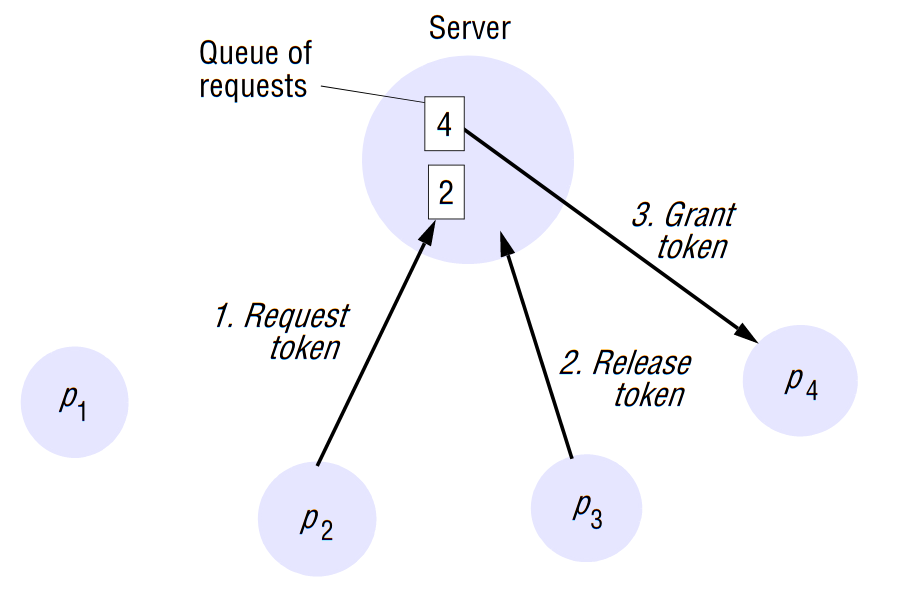
\includegraphics[width=0.5\textwidth]{central-server.png}}
  \caption{An example of the \textit{Central Server} algorithm}
\label{fig:central-server}
\end{figure}

\begin{figure}[htbp]
  \centerline{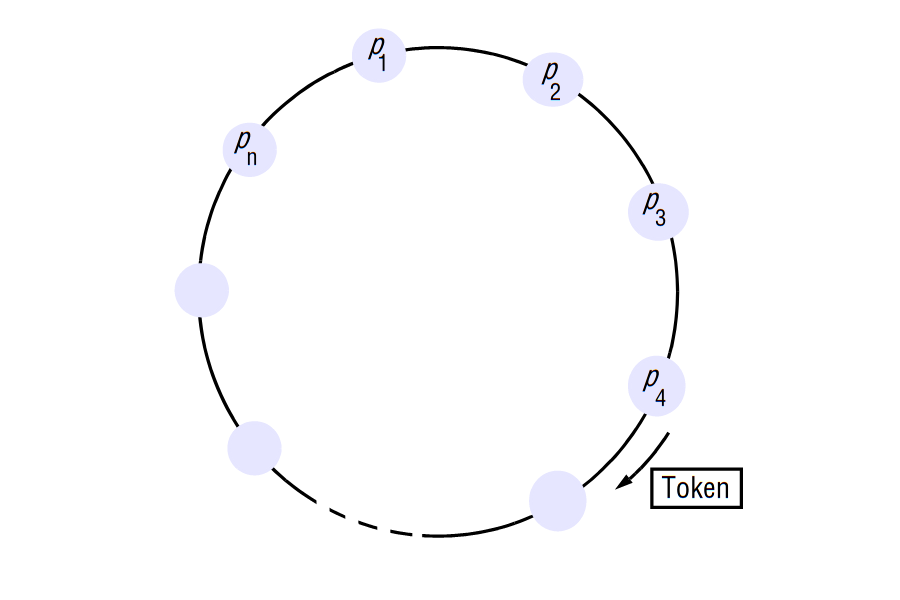
\includegraphics[width=0.5\textwidth]{ring-token.png}}
  \caption{The \textit{Ring Token} algorithm}
\label{fig:ring-token}
\end{figure}

\begin{figure*}[htbp]
  \centerline{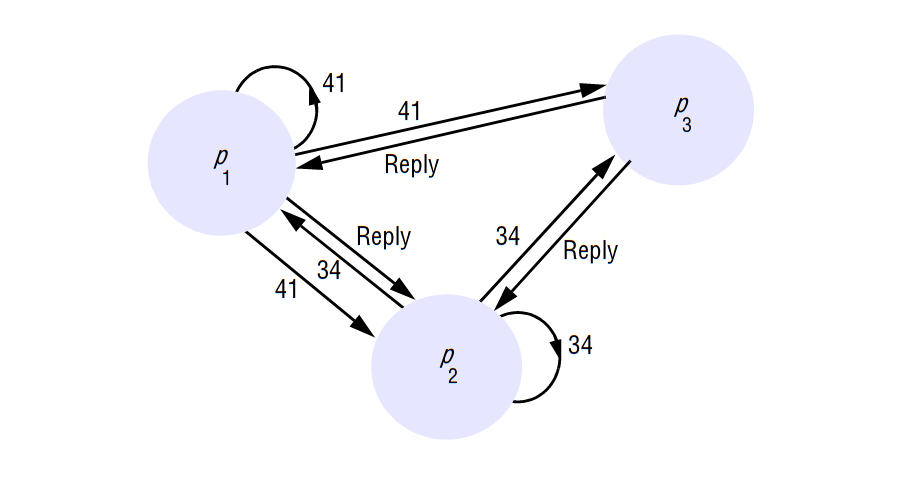
\includegraphics[width=1.0\textwidth]{multicast.png}}
  \caption{\large An example of the \textit{Multicast} algorithm}
\label{fig:multicast}
\end{figure*}

\section*{Acknowledgement}
This report acknowledges the teachings of Dr. Avinash Malik and Ms. Jesin James
in the course COMPSYS 725: Distributed Cyber-Physical Systems taught at the
University of Auckland in Semester Two of the year 2020.

\begin{thebibliography}{00}
\bibitem{b1} George F. Coulouris, Jean Dollimore, Tim Kindberg and Gordon
  Blair, ``Distributed Systems: Concepts and Designs'', 5th ed, Boston,
    Massachusetts, Addison-Wesley; Pearson Education, 2011, pp. 41-49.
\end{thebibliography}
\vspace{12pt}
\end{document}
